% !TEX root = arbeit.tex
\appendix
	
\section{Appendix}
	\subsection{Papers}
	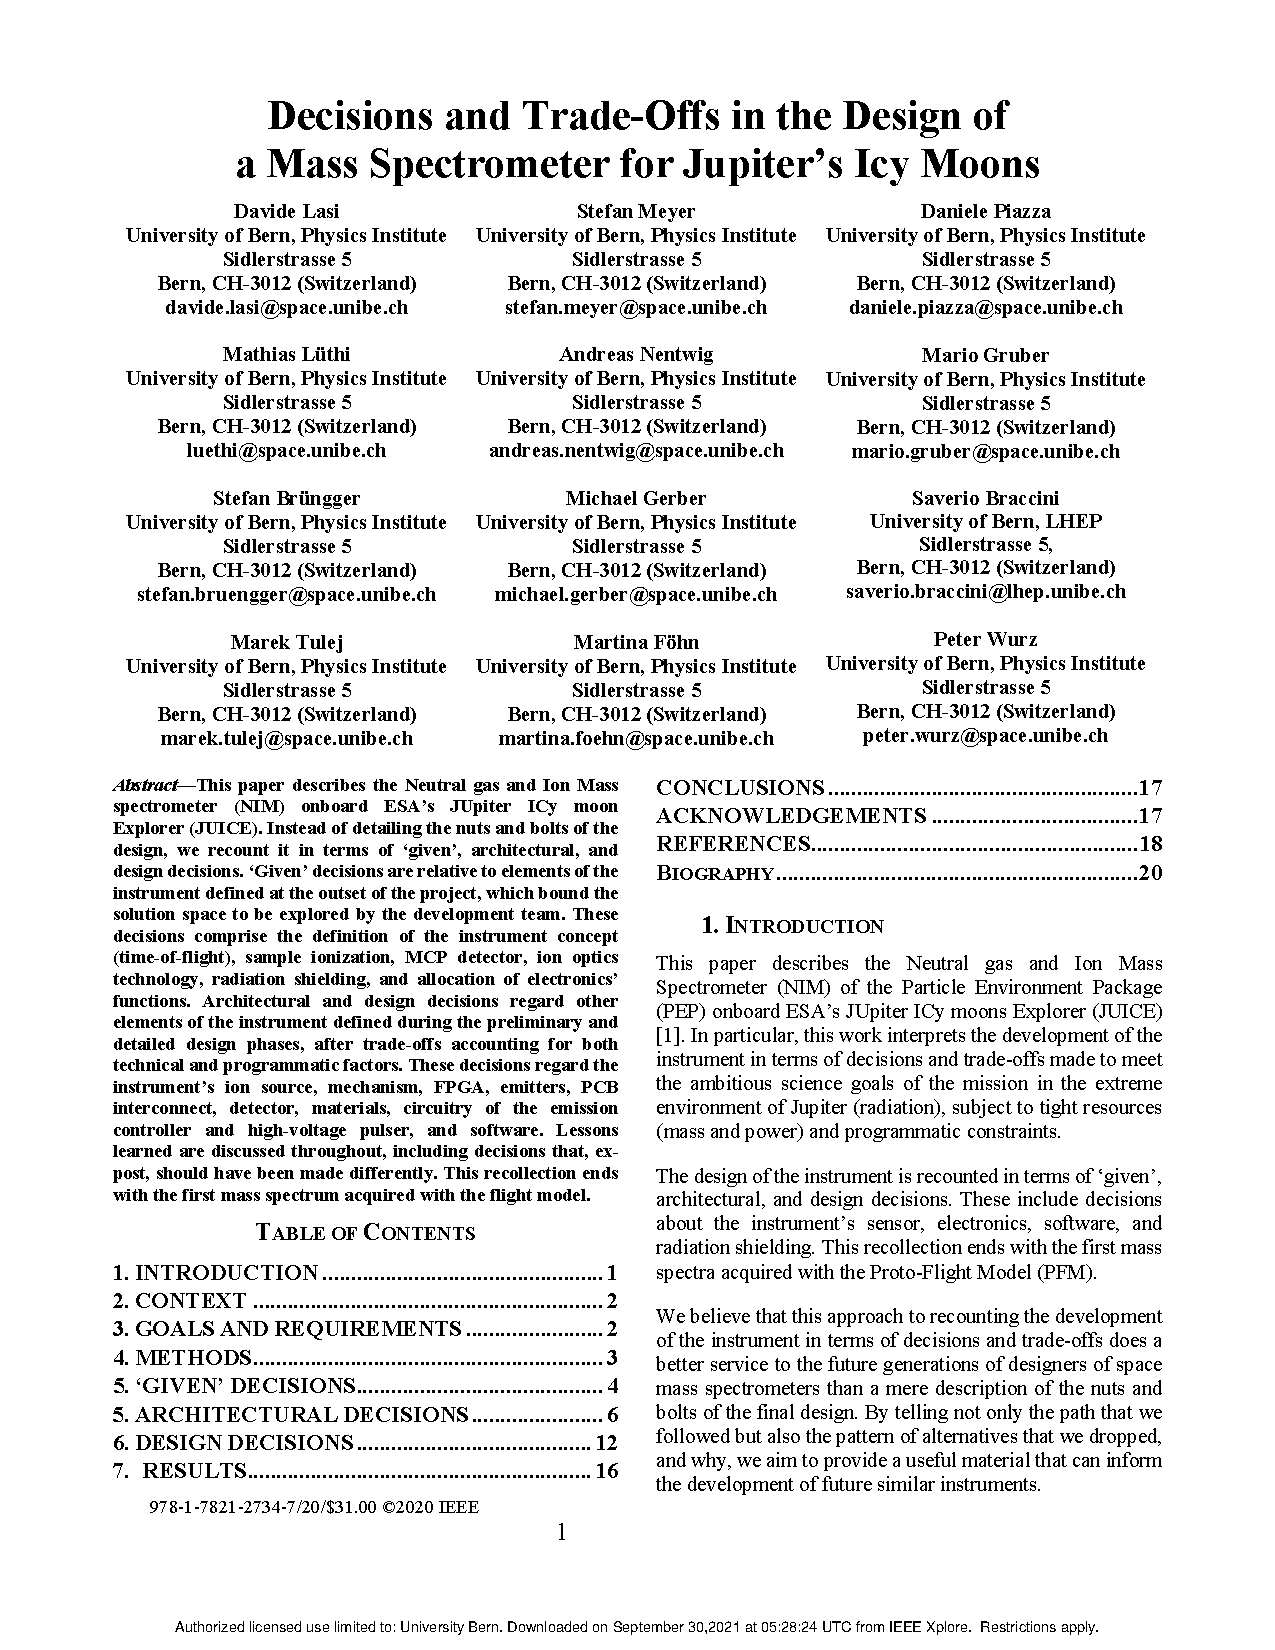
\includepdf[pages={1-}]{Lasi_2020_final.pdf}
	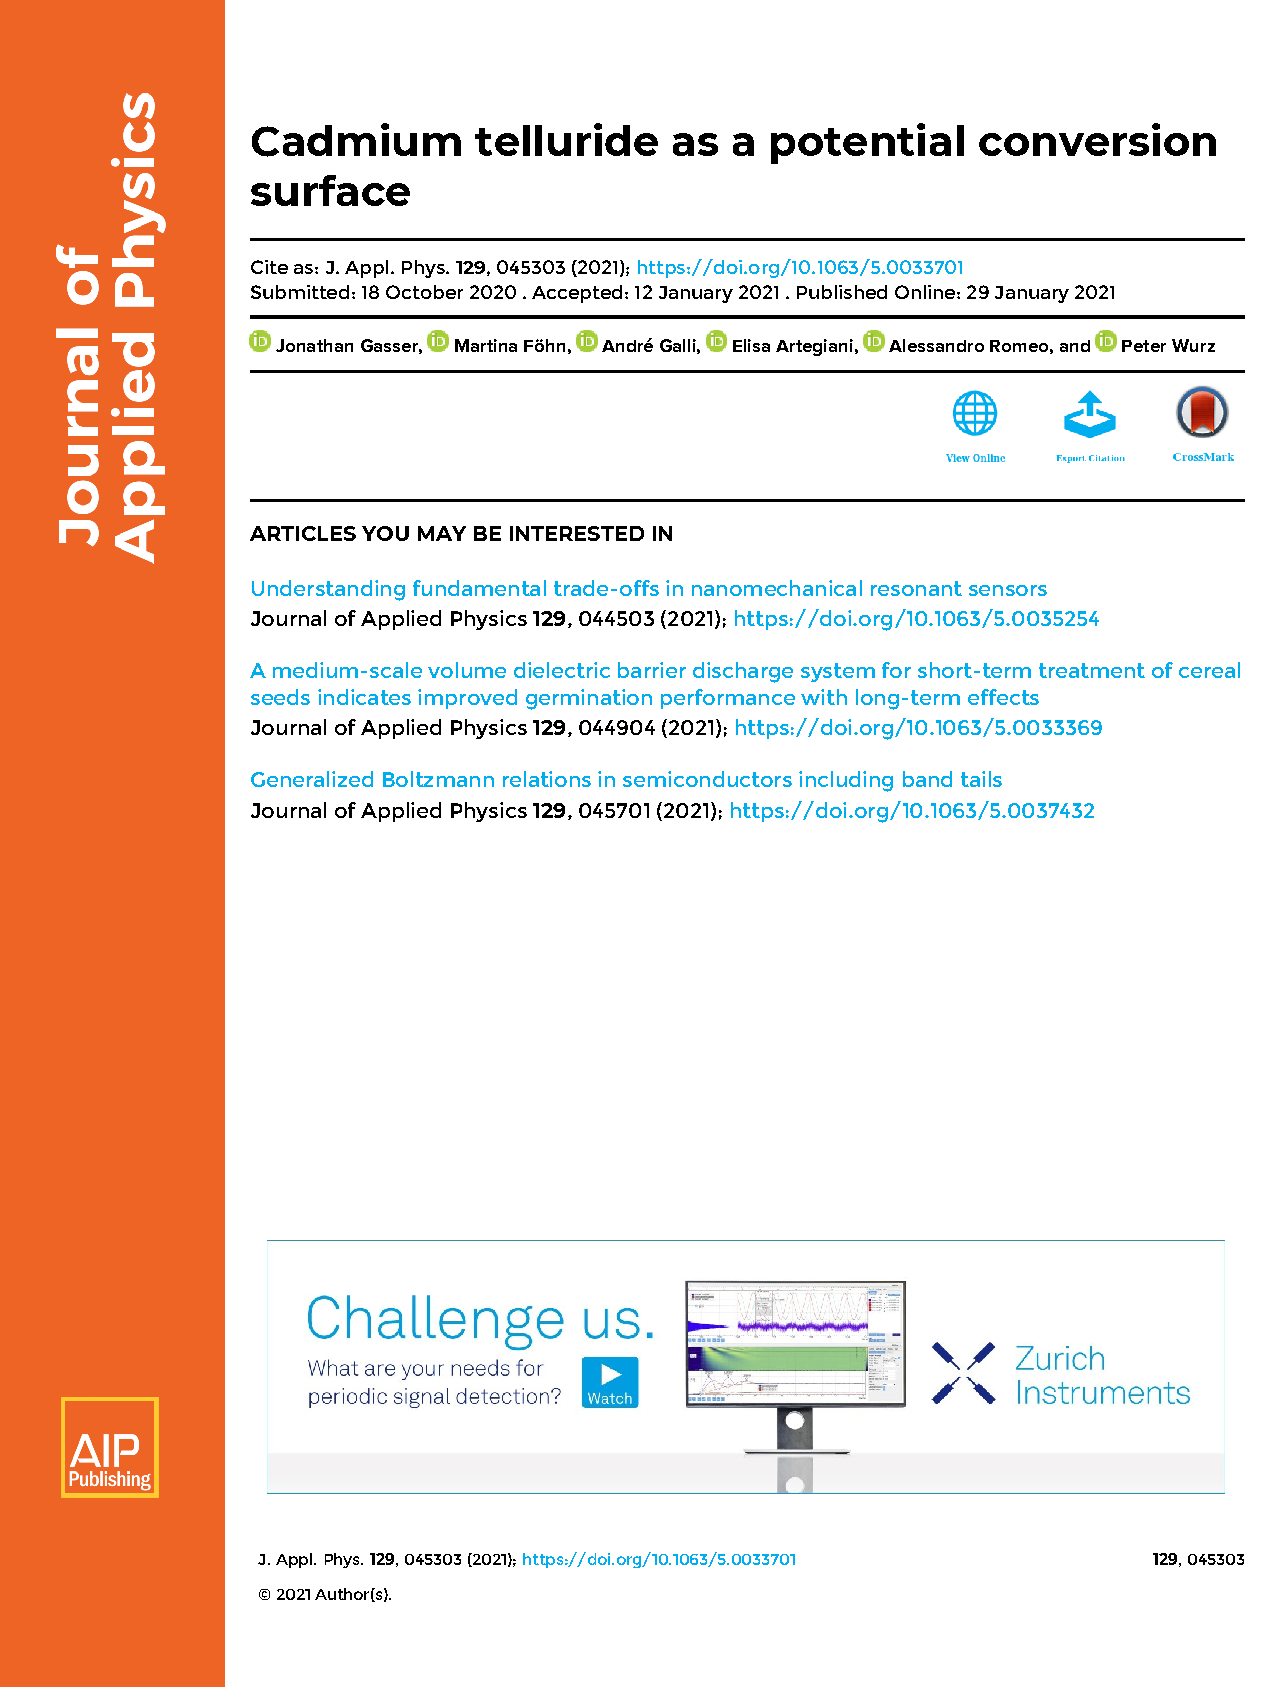
\includepdf[pages={1-}]{Gasser2021_CdTe.pdf}
	
	\subsection{Data sheets} \label{sec:appendix}
	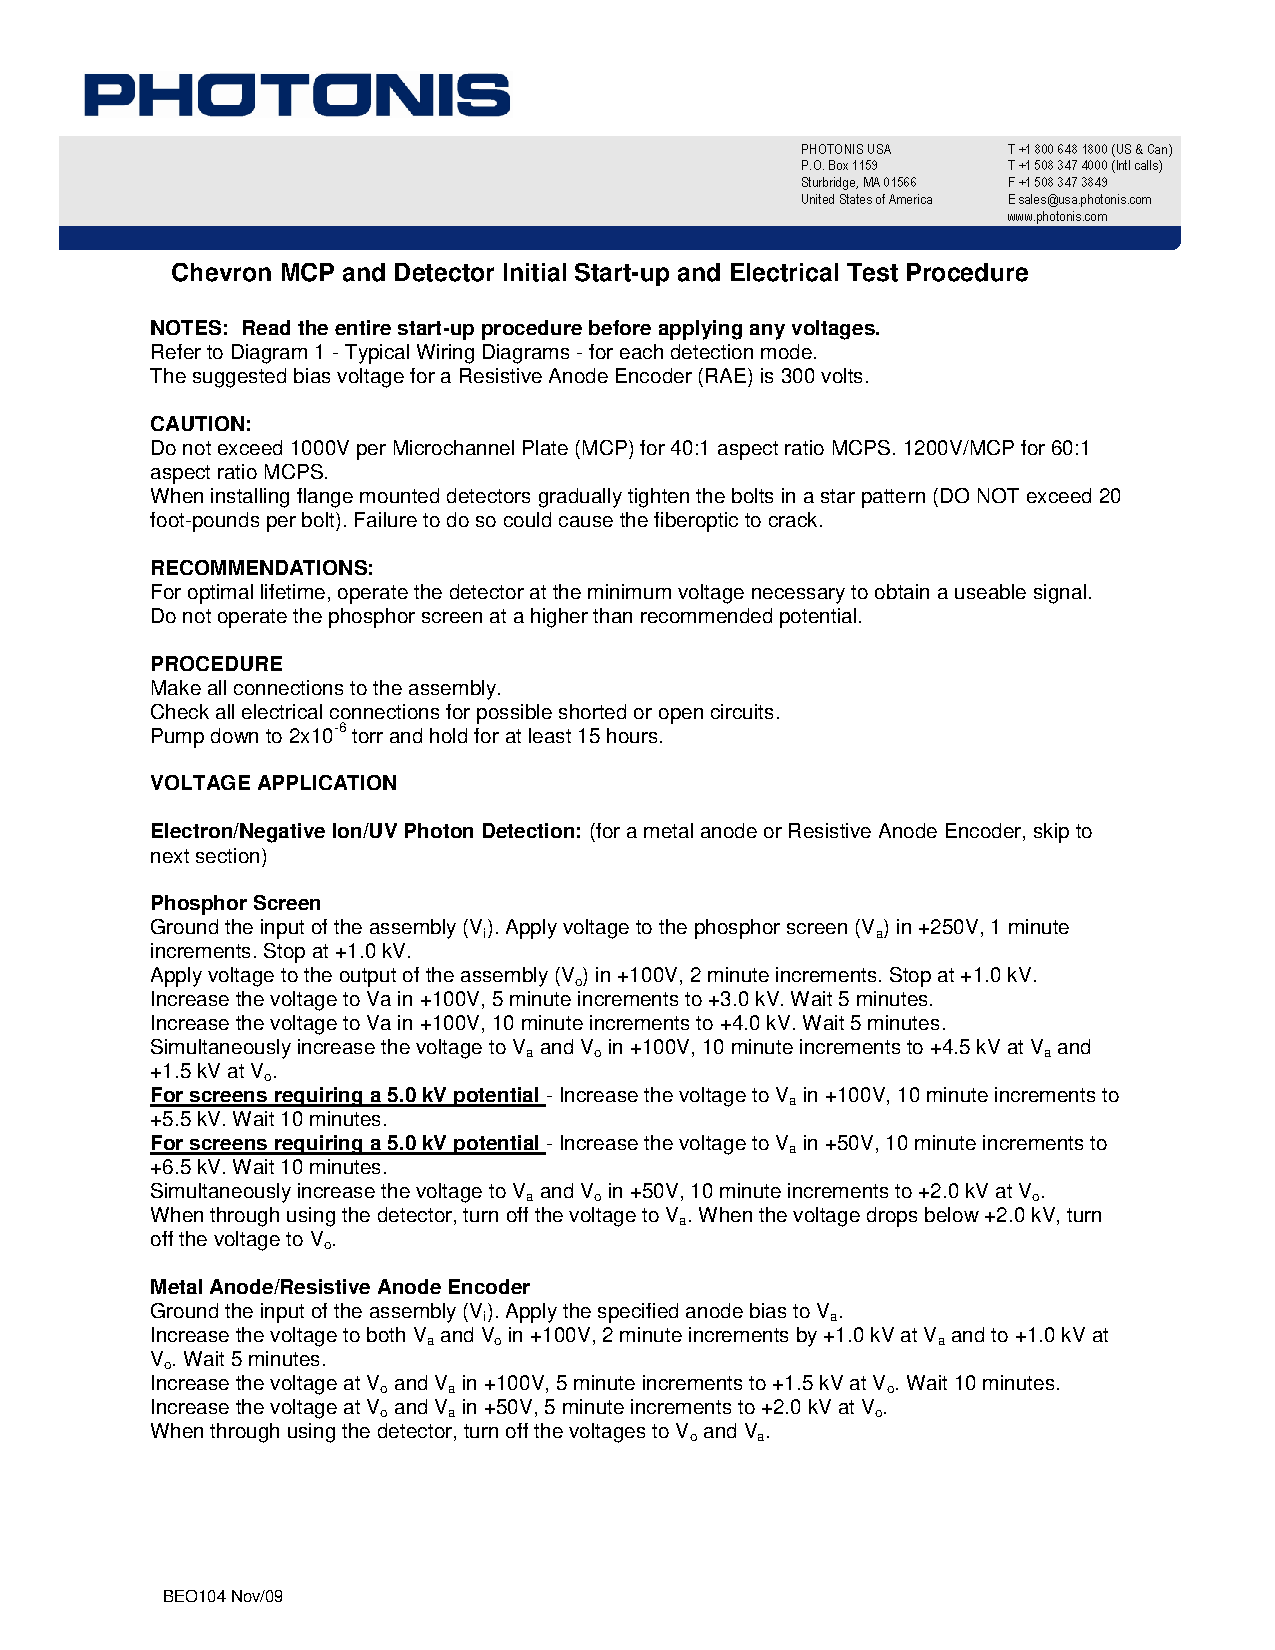
\includepdf[pages=-]{MCP_Startup_procedure.pdf}

	\subsection{Voltage Table} \label{VoltageSet}
	
	\begin{small}
	\begin{table}[H]
		\centering
		\begin{tabular}{|ll|rrrr|}
			\hline
			\textbf{\# electrode} & \textbf{name}   & \multicolumn{2}{c}{\textbf{PFM}} & \multicolumn{2}{c|}{\textbf{FS}} \\
			& & \textbf{th-Mode [V]} & \textbf{n-Mode [V]} & \textbf{th-Mode  [V]} & \textbf{n-Mode [V]} \\
			\hline
			IS 1          & push grid       &  -0.2 &    -1 &  -1.1 & -1.25 \\
			IS 2          & ion-repeller l  &   150 & 122.5 &   125 & 122.5 \\
			IS 3          & entrence        &    0 &      0 &     0 &     0 \\
			IS 4          & ion-repeller r  &   150 &   142 &   143 &   148 \\
			IS 5/6        & Pulser Bias     &     0 &     0 &   0.2 &   0.3 \\
			IS 5/6        & Pulser HV       &  -480 &  -480 &  -480 &  -480 \\
			IS 7          & lens 1          &  -300 &   182 & -1300 & -1500 \\
			IS 8          & lens 2          & -1800 & -2221 & -3400 & -3250 \\
			IS 9          & lens 3          & -1500 & -1150 & -1250 & -1750 \\
			IS 10         & lens 4          & -3200 & -1121 & -2125 & -2500 \\
			IS 11         & lens 5          & -1600 & -3565 & -2800 & -2500 \\
			IS 12         & lens 6          & -2400 & -1197 & -1750 & -1850 \\
			IS 13         & lens 7          & -3000 & -1573 & -5000 & -5000 \\
						  &                 &       &       &       &       \\
			R 2           & focusing        & -6450 & -5477 & -6600 & -6700 \\
			R 4           & retarding 1     &  -400 &   146 &     0 &   150 \\
			R 8           & intermediate    & -1200 & -1091 & -1035 & -1025 \\
			R 15          & backplane       &    20 &   -20 &   175 &   200 \\
						  &                 &       &       &       &       \\
			UMCP          &                 &  1850 &  1900 &  1900 &  1950 \\
			MCP Front/ D4 & D/ Front        & -2500 & -2600 & -2500 & -2500 \\
						  &                 &       &       &       &       \\
			FIL 1         & filament (bias) &   -70 &   -70 &   -70 &   -70 \\
			FIL 2         & e-repeller      &   -72 &   -70 &   -70 &   -70 \\
			FIL 3         & e-slit          &   110 &   104 &    95 &   100 \\
			\hline
		\end{tabular}
		\caption{Voltage sets for NIM PFM and FS instruments.}
		\label{tab:voltageSets}
	\end{table}
	\end{small}
